% A simple template for LaTeX documents
% 
% To produce pdf run:
%   $ pdflatex paper.tex 
%


\documentclass[12pt]{article}

% Begin paragraphs with new line
\usepackage{parskip}  

% Change margin size
\usepackage[margin=1in]{geometry}   

% Graphics Example:  (PDF's make for good plots)
\usepackage{graphicx}               
% \centerline{\includegraphics{figure.pdf}}

% subfigures, side by side
\usepackage{subcaption}

% hyperlinks
\usepackage{hyperref}

% Blocks of code
\usepackage{listings}
\lstset{basicstyle=\ttfamily, title=\lstname}
% Insert code like this. replace `plot.R` with file name.
% \lstinputlisting{plot.R}

% Monospaced fonts
%\usepackage{inconsolata}
% GNU \texttt{make} is a nice tool.

% Supports proof environment
\usepackage{amsthm}

% Allows writing \implies and align*
\usepackage{amsmath}

% Allows mathbb{R}
\usepackage{amsfonts}

% Numbers in scientific notation
% \usepackage{siunitx}

% Use tables generated by pandas
\usepackage{booktabs}

% Allows umlaut and non ascii characters
\usepackage[utf8]{inputenc}

% norm and infinity norm
\newcommand{\norm}[1]{\left\lVert#1\right\rVert}
\newcommand{\inorm}[1]{\left\lVert#1\right\rVert_\infty}

% Statistics essentials
\newcommand{\iid}{\text{ iid }}
\newcommand{\Exp}{\operatorname{E}}
\newcommand{\Var}{\operatorname{Var}}
\newcommand{\Cov}{\operatorname{Cov}}


%%%%%%%%%%%%%%%%%%%%%%%%%%%%%%%%%%%%%%%%%%%%%%%%%%%%%%%%%%%%

\begin{document}

\title{Selecting Sizes For Parallel Chunks}
\date{\today}
\author{Clark Fitzgerald}
\maketitle

\begin{abstract}

    This is a prospectus for distribution to the committee for PhD
    Qualifying Exam in June 2017.

\end{abstract}


\section{Introduction}
%%%%%%%%%%%%%%%%%%%%%%%%%%%%%%%%%%%%%%%%%%%%%%%%%%%%%%%%%%%%

What new things am I bringing to the table? My QE is in two months, time to
focus.

General idea- code analysis to detect and use parallelism. Determining and
using a chunking scheme based on (code, platform, data).

Looking at the different 

Broad idea- more separation between the high level language
and the implementation.

Some functions can be applied in a streaming manner, where they visit the
data. Can we detect these functions programmatically? If we can then this
gives free parallelism.


\section{Chunking Approaches to Large Data}
%%%%%%%%%%%%%%%%%%%%%%%%%%%%%%%%%%%%%%%%%%%%%%%%%%%%%%%%%%%%

Side note- why do we need chunking? What's wrong with exceeding limits of
memory and just swapping to disk? Swap space is typically around the same
size as memory. For example, my Ubuntu 16.04 desktop has 8GB of RAM and 8GB
of swap space on a spinning disk (not an SSD).

\begin{figure}
\centering
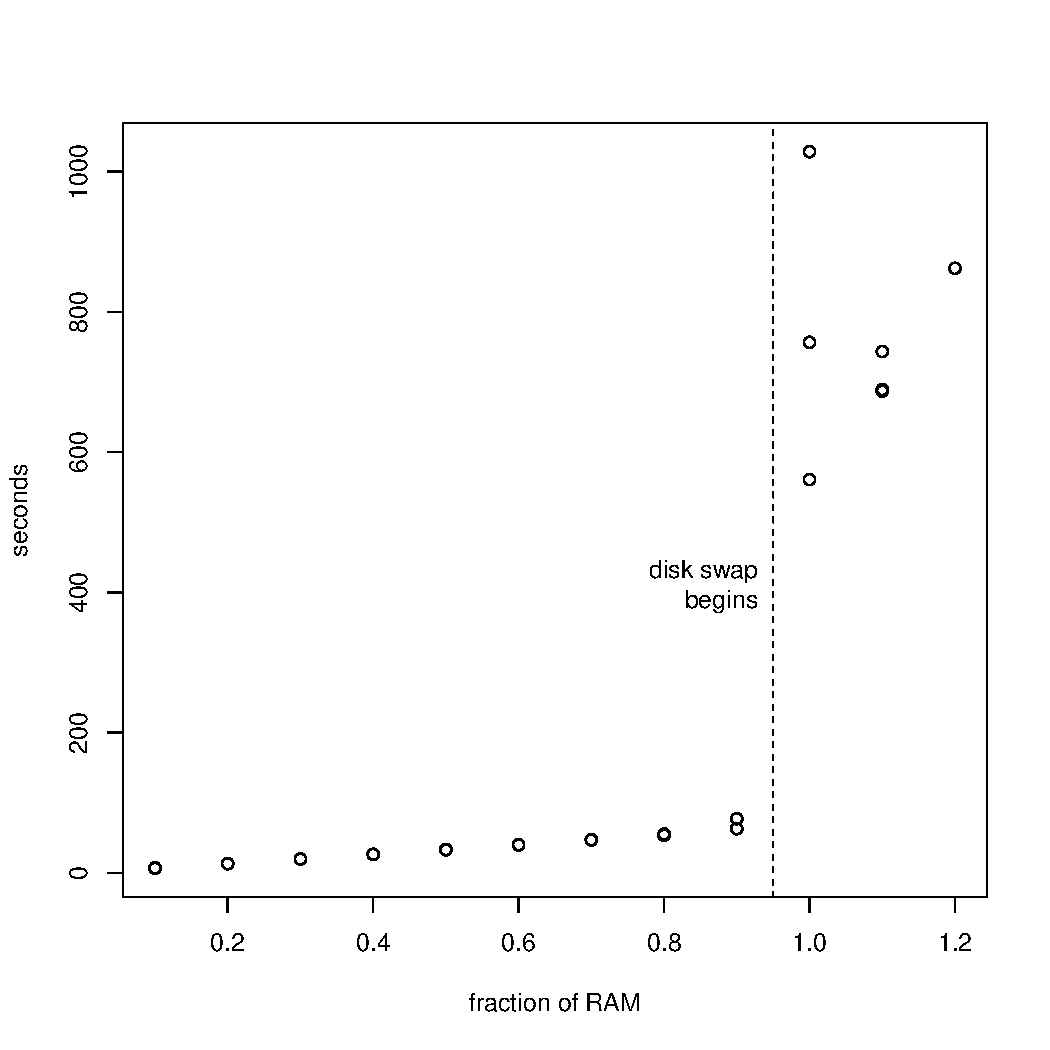
\includegraphics[width=.8\linewidth]{swap/spinning_disk_swap}
\caption{Performance is reasonable while data fits in memory.}
\label{fig:test}
\end{figure}



\textbf{Speculative evaluation of different chunked computation schemes}

A well known technique for parallel computation is to split data into
chunks and compute on each chunk simultaneously. This approach 
is useful on large data. Multiplying large block matrices is an example of this.

Many existing software packages for parallel computation requires one to specify the
chunk size. Examples include ddR \cite{R-ddR} and partools
\cite{R-partools} in R and dask in Python.
Yet chunk size strongly impacts
performance. If it's too small then there will be excessive overhead. If
it's too large then it won't fit into memory. In both cases performance
will suffer. But how much will it suffer?

Matloff presents compelling reasons to use a chunk based
approach for statistical applications \cite{matloff2014software}.

\subsection{Related Work}

Python's dask library infers appropriate block size for
\href{https://github.com/dask/dask/pull/1328}{reading CSV files}.

R's bigmemory package uses C++ and a memory mapped file which allows shared
memory access. \cite{kane2010bigmemory} It's a tool for representing large
data sets, and the package vignette mentions that chunking can and should
be used together when possible.

\subsection{Challenges}

For a given set of hardware and a given task graph in a given
computational model there may be
an optimal chunking scheme, or a range of chunk sizes with similar performance.
We'd like to automatically figure that out so the user doesn't have to
specify. It may be possible to gather data be speculatively running parts
of the computation and then using this as the inputs to a 
mathematical optimization problem.

I'd expect that a dynamic language calling vectorized C code has some set
of performance characteristics, while standalone C++ code is quite
different.
Extension: What chunking is optimal for GPU?

Allowing \texttt{rechunk()} operations in the middle of the task graph adds
much more flexibility and complexity. But it might be useful.

Need to be a little careful because the chunking scheme defines the dask
task graph. Then the semantics are more general than the dask graph. It's
really similar to optimization.

\subsection{Applications}

Google's TensorFlow can express large computational graphs on n dimensional
arrays (tensors), mostly for machine learning.

Apache Spark does chunking transparently to the user, and it's possible to
tune it for performance reasons.


\section{Chunking}

IDEA: nested parallelism- how to do it? If you hard code it in you're
stuck.

The task based parallelism isn't as relevant to how people use R (and other
languages) for data processing. Instead
lets think more about chunking and data parallelism. 

Parallelism introduces additional overhead on top of what dynamic languages
already incur. A general strategy to minimize this overhead is to ``chunk''
the computations. For example, given 1000 parallel operations one might
partition these into chunks of size 100 so that they become 10 parallel
tasks \cite{matloff2015parallel}.

I can take the code in \cite{matloff2015parallel} and see how changing the
chunk sizes affects the run time. I could also do this with Python's dask.
The goal is to draw general conclusions about which chunk sizes work best
based on the amount of computation.

It would be nice to run just a couple in serial on the master process and
make principled decisions about how to run based on these results. For
example:
\begin{itemize}
    \item Is it worth it to run in parallel?
    \item Should we chunk? What should the chunk sizes be?
    \item Reverse the order for better load balancing?
    \item Dynamic or static scheduling?
\end{itemize}

Usually none of these are known ahead of time.  They also depend on the
particular problem.  The only way to know if a chunking scheme will work is
to experiment with a similar problem, then check expectations for the next
one. I also expect that they vary across different machines.

The book mentions using large chunks in the beginning followed by small
chunks for superior load balancing.

Programming in the RDSM package conceptually is very similar to OpenCL on
the GPU. You allocate memory and send it to the workers, then update it in
place based on thread IDs. This is quite different than normal functional
R. I wonder if we could "translate" regular R into this style of
programming?

TODO: Come up with application where I need all this!! How about computing
graphs from Euclidean space like with James' application? It would be nice
for the QE to have something that he's familiar with and invested in.

\section{Software Alchemy}

Looking at Norm's book now. He mentions tuning Software Alchemy for
statistical purposes through chunk size. But I've been thinking about just
tuning them for computational efficiency. Perhaps these two different
lenses could be combined?

\section{Applications}

Goal: Fit a piecwise linear fundamental diagram for each station ID using 30 second
data. Fit using robust regression to limit the effect of outliers.
Each file is around 1 GB when loaded in R, and there are several hundred
files (we could actually take as many as we like). So this is beyond
the limits of what we can do in memory even on a server.

This can't be easily done in a database because robust regression is
a relatively specialized method, yet available in MASS::rlm.
Ideally we could combine the best of both worlds.

This is difficult because the data files are split by day, yet we
need to group by station ID, which shows up in every day.

Now I'm thinking about how to do this split. The ff package looks
appealing, but unmaintained for a little while. iotools and data.table
are also appealing to get high performance read / write. Let's see if I
can do this split with iotools pipeline parallelism

I could perform a file based split in several ways- with Spark, dask, and
rolling my own in R. I suspect that dask or R will be the easiest.

R- Advantage is that one can stay in the same system as where the analysis
will be done. 

Dask- Probably performs well

Spark- Putting the data into the SQL database would be pretty nice for
future work.

First I should do it one way. Let's go with R since I've already started.
I did the file based split with base R, no parallelism and it took 1402 minutes = 23.4 hours.

Big Data:

Norm was talking about the buzz around Hadoop mostly being a lot of hype.
Simon Urbanek processes crazy amounts of data using just plain old R.

\emph{While “Big Data” tools can be exciting, they are almost always worse than
normal data tools while those remain appropriate.} - Dask documentation

One problem is that moving to an entirely different system can require
completely rethinking your approach. dplyr and sparklyr are appealing in this
aspect because they basically use the same user API and do the right
thing at the backend. As with SQL, they're also more high level / descriptive of the
desired operation. Then we have this tension between simple code and
complex code. The simple code is easier to maintain and understand, while
the complex code is adapted to the system / problem at hand. A high level
idea is to take the simple code and make it perform as well or better than
the complex code necessary to run it in a more sophisticated way- ie. on a
parallel machine or a GPU.

In general one doesn't want to think about the chunks. At all.

A personal frustration I've experienced with the database type R interfaces
is that it's not possible to directly write user defined R that will work.
Most R / database interfaces that I've seen essentially allow one to do the
same thing in R as one could do in SQL. This is not helpful for me, because
I could just write the SQL myself. I use R not because I love the syntax,
rather I want the convenient and correct statistical functionality.

\section{Streams}

Thinking about the streaming example. Can we look at a
piece of code and determine if it can be converted to a streaming function?
This can be done for functions that are vectorized, ie. they compute things
elementwise. It can be done for functions that use a for loop over the
indices. 

It can't be done for more complex operations like sorting.

How about for compositions of streaming functions? Sure, this amounts to
loop fusion.

Reducing

\section{Examples}

Consider making a prediction vector for some $n \times p$ matrix $X$. This
is embarrassingly parallel since each row is independent. Suppose $X$ is on
disk, and super large- say $n = 1e10$ and $p = 3$. Then we want to 

\section{Disk based storage}

I'm noticing many different exciting options when it comes to serializing /
deserializing and binary storage of matrices and data frames.

I wonder if there's some way to combine and or unify these different
packages. It's very similar to what ddR tried to do. One could have an
abstract disk based dataframe with high performance. But the partools package already does
something quite similar. 


\begin{itemize}
    \item CSV - The ol' standby
    \item RDS - R's default binary serialization
    \item feather - Apache sponsored project, interopable between R /
        Python
    \item netCDF - binary storage of arrays with various levels of
        compression
    \item iotools - high 
    \item data.table - Arun Srinivasan's Sep 16 talk in Budapest helpful
        for understanding.

\end{itemize}



Many of these can use threads, which means they can potentially effectively
utilize all the CPU resources so that any multiprocessing becomes a hindrance.
Others, notably many of the base R functions, focus more on robustness than
performance. Then parallel processing is one way to improve things.

TODO: ask Norm- how does partools rely on data.table? data.table uses
threads to great effect, while partools uses SNOW clusters. It seems like
this would have the problem mentioned above if ran on the same machine.

\bibliographystyle{plain}
\bibliography{../citations,../Rpackages} 

\end{document}
